\documentclass[journal,12pt,twocolumn]{IEEEtran}
\usepackage{setspace}
\usepackage{gensymb}
\singlespacing
\usepackage[cmex10]{amsmath}
\usepackage{amsthm}
\usepackage{mathrsfs}
\usepackage{txfonts}
\usepackage{stfloats}
\usepackage{bm}
\usepackage{cite}
\usepackage{cases}
\usepackage{subfig}
\usepackage{longtable}
\usepackage{multirow}
\usepackage{enumitem}
\usepackage{mathtools}
\usepackage{steinmetz}
\usepackage{tikz}
\usepackage{circuitikz}
\usepackage{verbatim}
\usepackage{tfrupee}
\usepackage[breaklinks=true]{hyperref}
\usepackage{tkz-euclide}
\usetikzlibrary{calc,math}
\usepackage{listings}
    \usepackage{color}                                            %%
    \usepackage{array}                                            %%
    \usepackage{longtable}                                        %%
    \usepackage{calc}                                             %%
    \usepackage{multirow}                                         %%
    \usepackage{hhline}                                           %%
    \usepackage{ifthen}                                           %%
  %optionally (for landscape tables embedded in another document): %%
    \usepackage{lscape}     
\usepackage{multicol}
\usepackage{chngcntr}
\DeclareMathOperator*{\Res}{Res}
\renewcommand\thesection{\arabic{section}}
\renewcommand\thesubsection{\thesection.\arabic{subsection}}
\renewcommand\thesubsubsection{\thesubsection.\arabic{subsubsection}}

\renewcommand\thesectiondis{\arabic{section}}
\renewcommand\thesubsectiondis{\thesectiondis.\arabic{subsection}}
\renewcommand\thesubsubsectiondis{\thesubsectiondis.\arabic{subsubsection}}

% correct bad hyphenation here
\hyphenation{op-tical net-works semi-conduc-tor}
\def\inputGnumericTable{}                                 %%

\lstset{
frame=single, 
breaklines=true,
columns=fullflexible
}

\begin{document}


\newtheorem{theorem}{Theorem}[section]
\newtheorem{problem}{Problem}
\newtheorem{proposition}{Proposition}[section]
\newtheorem{lemma}{Lemma}[section]
\newtheorem{corollary}[theorem]{Corollary}
\newtheorem{example}{Example}[section]
\newtheorem{definition}[problem]{Definition}
\newcommand{\BEQA}{\begin{eqnarray}}
\newcommand{\EEQA}{\end{eqnarray}}
\newcommand{\define}{\stackrel{\triangle}{=}}

\bibliographystyle{IEEEtran}
\providecommand{\mbf}{\mathbf}
\providecommand{\pr}[1]{\ensuremath{\Pr\left(#1\right)}}
\providecommand{\qfunc}[1]{\ensuremath{Q\left(#1\right)}}
\providecommand{\sbrak}[1]{\ensuremath{{}\left[#1\right]}}
\providecommand{\lsbrak}[1]{\ensuremath{{}\left[#1\right.}}
\providecommand{\rsbrak}[1]{\ensuremath{{}\left.#1\right]}}
\providecommand{\brak}[1]{\ensuremath{\left(#1\right)}}
\providecommand{\lbrak}[1]{\ensuremath{\left(#1\right.}}
\providecommand{\rbrak}[1]{\ensuremath{\left.#1\right)}}
\providecommand{\cbrak}[1]{\ensuremath{\left\{#1\right\}}}
\providecommand{\lcbrak}[1]{\ensuremath{\left\{#1\right.}}
\providecommand{\rcbrak}[1]{\ensuremath{\left.#1\right\}}}
\theoremstyle{remark}
\newtheorem{rem}{Remark}
\newcommand{\sgn}{\mathop{\mathrm{sgn}}}
\providecommand{\abs}[1]{\left\vert#1\right\vert}
\providecommand{\res}[1]{\Res\displaylimits_{#1}} 
\providecommand{\norm}[1]{\left\lVert#1\right\rVert}
\providecommand{\mtx}[1]{\mathbf{#1}}
\providecommand{\mean}[1]{E\left[ #1 \right]}
\providecommand{\fourier}{\overset{\mathcal{F}}{ \rightleftharpoons}}
\providecommand{\system}{\overset{\mathcal{H}}{ \longleftrightarrow}}
\newcommand{\solution}{\noindent \textbf{Solution: }}
\newcommand{\cosec}{\,\text{cosec}\,}
\providecommand{\dec}[2]{\ensuremath{\overset{#1}{\underset{#2}{\gtrless}}}}
\newcommand{\myvec}[1]{\ensuremath{\begin{pmatrix}#1\end{pmatrix}}}
\newcommand{\mydet}[1]{\ensuremath{\begin{vmatrix}#1\end{vmatrix}}}
\numberwithin{equation}{subsection}
\makeatletter
\@addtoreset{figure}{problem}
\makeatother

\let\StandardTheFigure\thefigure
\let\vec\mathbf
\renewcommand{\thefigure}{\theproblem}



\def\putbox#1#2#3{\makebox[0in][l]{\makebox[#1][l]{}\raisebox{\baselineskip}[0in][0in]{\raisebox{#2}[0in][0in]{#3}}}}
     \def\rightbox#1{\makebox[0in][r]{#1}}
     \def\centbox#1{\makebox[0in]{#1}}
     \def\topbox#1{\raisebox{-\baselineskip}[0in][0in]{#1}}
     \def\midbox#1{\raisebox{-0.5\baselineskip}[0in][0in]{#1}}

\vspace{3cm}


\title{Assignment 1}
\author{Jaswanth Chowdary Madala}





% make the title area
\maketitle

\newpage

%\tableofcontents

\bigskip

\renewcommand{\thefigure}{\theenumi}
\renewcommand{\thetable}{\theenumi}

\begin{enumerate}
\item A ray of light passing through the point $\brak{1, 2}$ reflects on the x-axis at point A and the reflected ray passes through the point $\brak{5, 3}$. Find the coordinates of A.

\begin{figure}[ht]
\centering
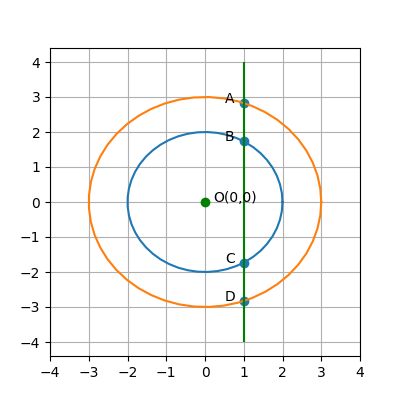
\includegraphics[width = \columnwidth]{"./figs/fig.png"}
\caption{Graph}
\label{fig:1}
\end{figure}

\textbf{Solution:} 
\begin{enumerate}
\item Expression for reflection of a point $\vec{P}$ in the line $\vec{n}^{\top}\vec{x} = c$.

Let the reflected point be $\vec{Q}$. The point $\vec{Q}$ can be written in parametric form as,
\begin{align}
\vec{Q} &= \vec{P} + \lambda\vec{n}
\end{align}
The points $\vec{P}$,$\vec{Q}$ are both equidistant from the line $\vec{n}^{\top}\vec{x} = c$. The point $\frac{\vec{P}+\vec{Q}}{2}$ lies on the line.
\begin{align}
\vec{n}^{\top}\brak{\frac{\vec{P}+\vec{Q}}{2}} &= c\\
\vec{n}^{\top}\brak{\frac{2\vec{P}+\lambda\vec{n}}{2}} &= c\\
2\vec{n}^{\top}\vec{P}+\lambda\vec{n}^{\top}\vec{n} &= 2c\\
\lambda &= -\frac{2\brak{\vec{n}^{\top}\vec{P}-c}}{\norm{\vec{n}}}
\end{align}
Hence, the point $\vec{Q}$ is given by,
\begin{align}
\vec{Q} &= \vec{P} -\frac{2\brak{\vec{n}^{\top}\vec{P}-c}}{\norm{\vec{n}}}\vec{n}
\end{align}

\item Let the points be,
\begin{align}
\vec{P} = \myvec{1\\2}, \, \vec{Q} = \myvec{5\\3}
\end{align}
The equation of $x$-axis is given by,
\begin{align}
\myvec{0&1}\vec{x} = 0
\end{align}
Let the reflection of point $\vec{Q}$ in the $x$-axis be $\vec{R}$ is given by
\begin{align}
\vec{R} &= \vec{Q} -\frac{2\brak{\vec{n}^{\top}\vec{Q}-c}}{\norm{\vec{n}}}\vec{n}\\
&= \myvec{5\\3} - 6\myvec{0\\1}\\
&= \myvec{5\\-3}
\end{align}
The point $\vec{A}$ is the point of intersection of the line $PR$ and $x$-axis.

Direction vector of line $PR$ is given by,
\begin{align}
\vec{m} &= \vec{R} - \vec{P}\\
&= \myvec{5\\-3} - \myvec{1\\2}\\
&= \myvec{4\\-5}
\end{align}
Normal vector $\vec{n}$ is given by,
\begin{align}
\vec{n} &= \myvec{5\\4}
\end{align}
Equation of line $PR$ is given by
\begin{align}
\myvec{5&4}\vec{x} &= \myvec{5&4}\myvec{1\\2}\\
\myvec{5&4}\vec{x} &= 13
\label{eq:1}\\
\vec{A} &= \myvec{x\\0}
\end{align}
The point $\vec{A}$ satisfies the equation \eqref{eq:1}
\begin{align}
5\times x &= 13\\
x &= \frac{13}{5}
\end{align}
Hence the point $\vec{A}$ is given by,
\begin{align}
\vec{A} = \myvec{\frac{13}{5}\\0}
\end{align}
\end{enumerate}
\end{enumerate}
\end{document}



